%%
%% This is file `hustreport-en-example.tex',
%% generated with the docstrip utility.
%%
%% The original source files were:
%%
%% hustreport.dtx  (with options: `example-en')
%% 
%% This is a generated file.
%% 
%% Copyright (C) 2013-2014 by Xu Cheng <xucheng@me.com>
%%               2014-2016 by hust-latex <https://github.com/hust-latex>
%% 
%% This work may be distributed and/or modified under the
%% conditions of the LaTeX Project Public License, either version 1.3
%% of this license or (at your option) any later version.
%% The latest version of this license is in
%%   http://www.latex-project.org/lppl.txt
%% and version 1.3 or later is part of all distributions of LaTeX
%% version 2005/12/01 or later.
%% 
%% This work has the LPPL maintenance status `maintained'.
%% 
%% The Current Maintainer of this work is hust-latex Organization.
%% 
%% This work consists of the files hustreport.dtx,
%% hustreport.ins and the derived file hustreport.cls
%% along with its document and example files.
%% 
%% \CharacterTable
%% {Upper-case    \A\B\C\D\E\F\G\H\I\J\K\L\M\N\O\P\Q\R\S\T\U\V\W\X\Y\Z
%%  Lower-case    \a\b\c\d\e\f\g\h\i\j\k\l\m\n\o\p\q\r\s\t\u\v\w\x\y\z
%%  Digits        \0\1\2\3\4\5\6\7\8\9
%%  Exclamation   \!     Double quote  \"     Hash (number) \#
%%  Dollar        \$     Percent       \%     Ampersand     \&
%%  Acute accent  \'     Left paren    \(     Right paren   \)
%%  Asterisk      \*     Plus          \+     Comma         \,
%%  Minus         \-     Point         \.     Solidus       \/
%%  Colon         \:     Semicolon     \;     Less than     \<
%%  Equals        \=     Greater than  \>     Question mark \?
%%  Commercial at \@     Left bracket  \[     Backslash     \\
%%  Right bracket \]     Circumflex    \^     Underscore    \_
%%  Grave accent  \`     Left brace    \{     Vertical bar  \|
%%  Right brace   \}     Tilde         \~}
\documentclass[language=english,category=academic-report]{hustreport}

\stuno{U2009xxxxx}
\title{An Example of Using hustreport \LaTeX{} Template}
\author{Xu Cheng}
\major{Electronic and Information Engineering}
\department{Electronic and Information Engineering}
\advisor{Ass. Prof. Xiaojun Hei}


\abstract{
    This is a \LaTeX{} template example file. This template is used in written thesis for Huazhong Univ. of Sci. \& Tech.

    This template is published under LPPL v1.3 License.

}
\keywords{\LaTeX{}, Huazhong Univ. of Sci. \& Tech., Report, Template}

\begin{document}

\frontmatter
\maketitle
\makeabstract
\tableofcontents
\listoffigures
\listoftables
\mainmatter

\chapter{Simple Test}\label{chapter:1}

\section{Level 1}\label{sec:1}
\subsection{Level 2}\label{sec:2}
\subsubsection{Level 3}\label{sec:3}
Content
\footnote{\label{footnote:1}A footnote.}

\section{Font}

Normal \textbf{Bold} \emph{Italic} \textsf{Sans}

The quick brown fox jumps over the lazy dog.

\section{Equation}

Single equation, see \autoref{eq:1}.
\begin{equation}
  c^2 = a^2 + b^2 \label{eq:1}
\end{equation}

Multi-equations, see \autoref{eq:2} and \autoref{eq:3}.

\begin{subequations}
\begin{equation}
  F = ma \label{eq:2}
\end{equation}
\begin{equation}
  E = mc^2 \label{eq:3}
\end{equation}
\end{subequations}

\section{List Environment}

\begin{enumerate}
    \item Level 1\label{item:1}
    \item Level 1
    \begin{enumerate}
        \item Level 2\label{item:2}
        \item Level 2
        \begin{enumerate}
            \item Level 3\label{item:3}
            \item Level 3
        \end{enumerate}
    \end{enumerate}
\end{enumerate}

\begin{description}
    \item[Discription]  Content
\end{description}

\chapter{Other Test}

\section{Code Highlight}

\begin{lstlisting}[language=python]
import os

def main():
    '''
    doc here
    '''
    print 'hello, world' # Abc
\end{lstlisting}

\section{Theorem}

\begin{definition}\label{def:1}
This is a definition.
\end{definition}
\begin{proposition}\label{proposition:1}
This is a proposition.
\end{proposition}
\begin{axiom}\label{axiom:1}
This is an axiom.
\end{axiom}
\begin{lemma}\label{lemma:1}
This is a lemma.
\end{lemma}
\begin{theorem}\label{theorem:1}
This is a theorem.
\end{theorem}
\begin{proof}\label{proof:1}
This is a proof.
\end{proof}

\section{Algorithm}

\begin{algorithm}[H]
\SetAlgoLined
\KwData{this text}
\KwResult{how to write algorithm with \LaTeX2e }
initialization\;\label{alg_line:1}
\While{not at end of this document}{
read current\;
\eIf{understand}{
go to next section\;
current section becomes this one\;
}{
go back to the beginning of current section\;
}
}
\caption{How to write algorithms}\label{alg:1}
\end{algorithm}

\section{Table}
See \autoref{tab:1}.

\begin{table}[!h]
\centering
\caption{A table}\label{tab:1}
\begin{tabular}{|c|c|}
\hline
a & b \\
\hline
c & d \\
\hline
\end{tabular}
\end{table}

\section{Figure}
See \autoref{fig:1}.Figure supports format in eps, png, pdf and so on. Multi-figures, see \autoref{fig:2}. Reference separately: \autoref{fig:2-1}, \autoref{fig:2-2}.

\begin{figure}[!h]
\centering
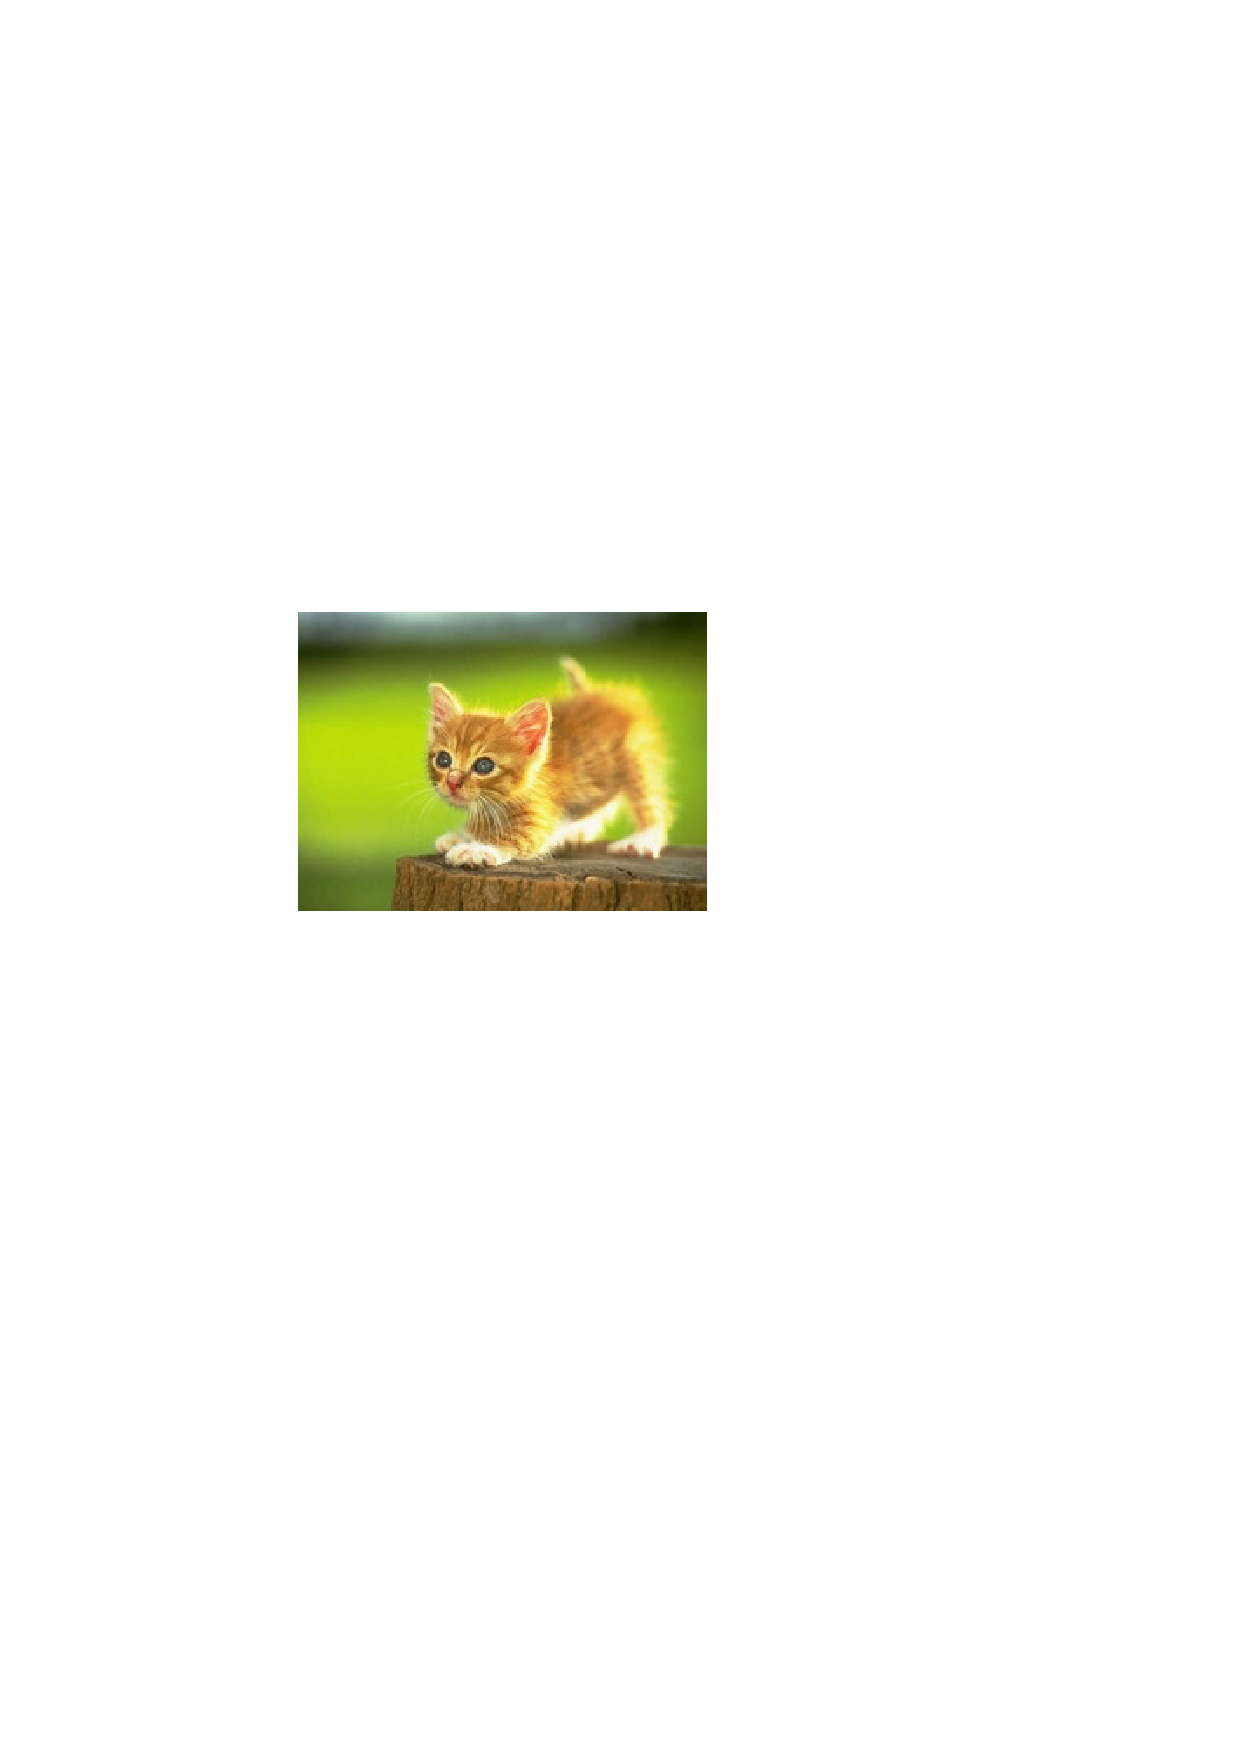
\includegraphics[width=.4\textwidth]{fig-example.pdf}
\caption{A figure}\label{fig:1}
\end{figure}

\begin{figure}[!h]
\centering
  \begin{subfigure}[b]{0.3\textwidth}
  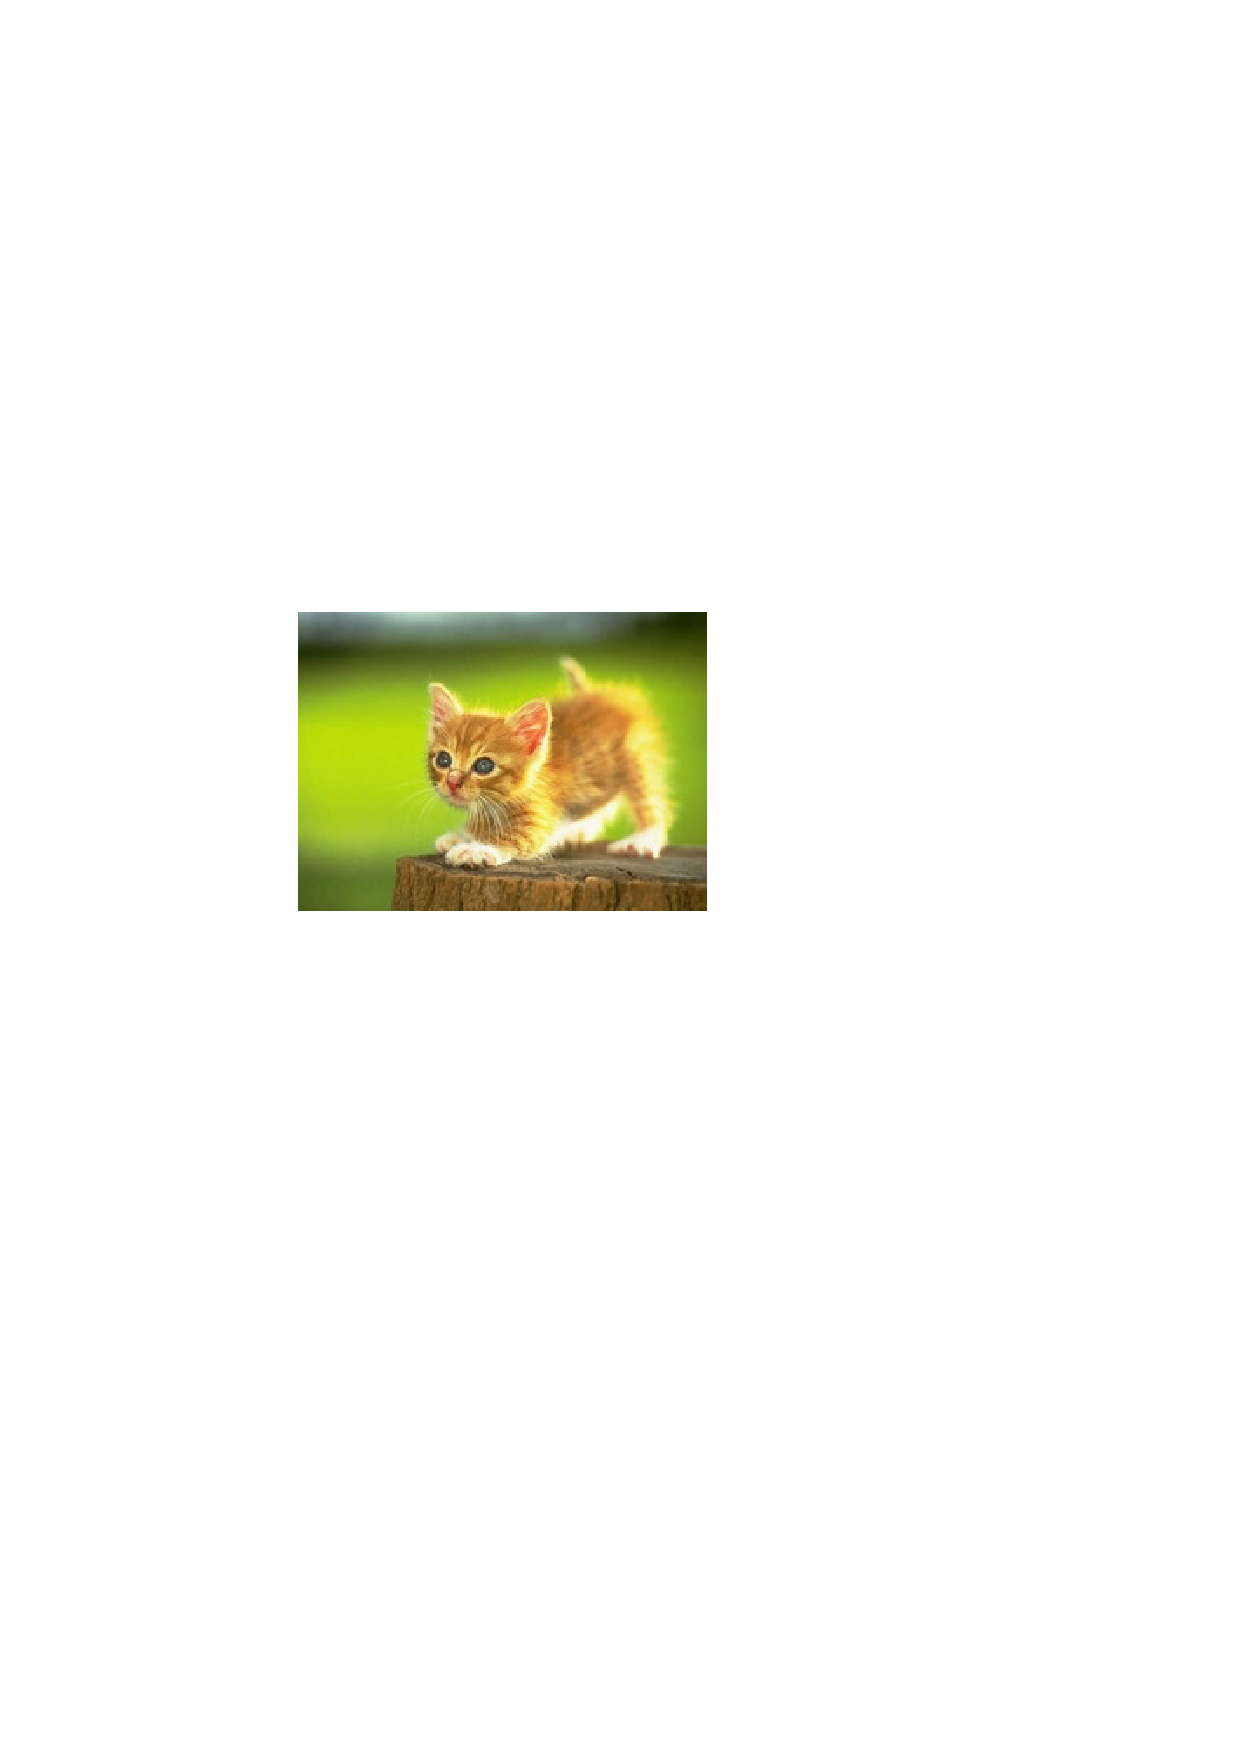
\includegraphics[width=\textwidth]{fig-example.pdf}
  \caption{Figure A}\label{fig:2-1}
  \end{subfigure}
  ~
  \begin{subfigure}[b]{0.3\textwidth}
  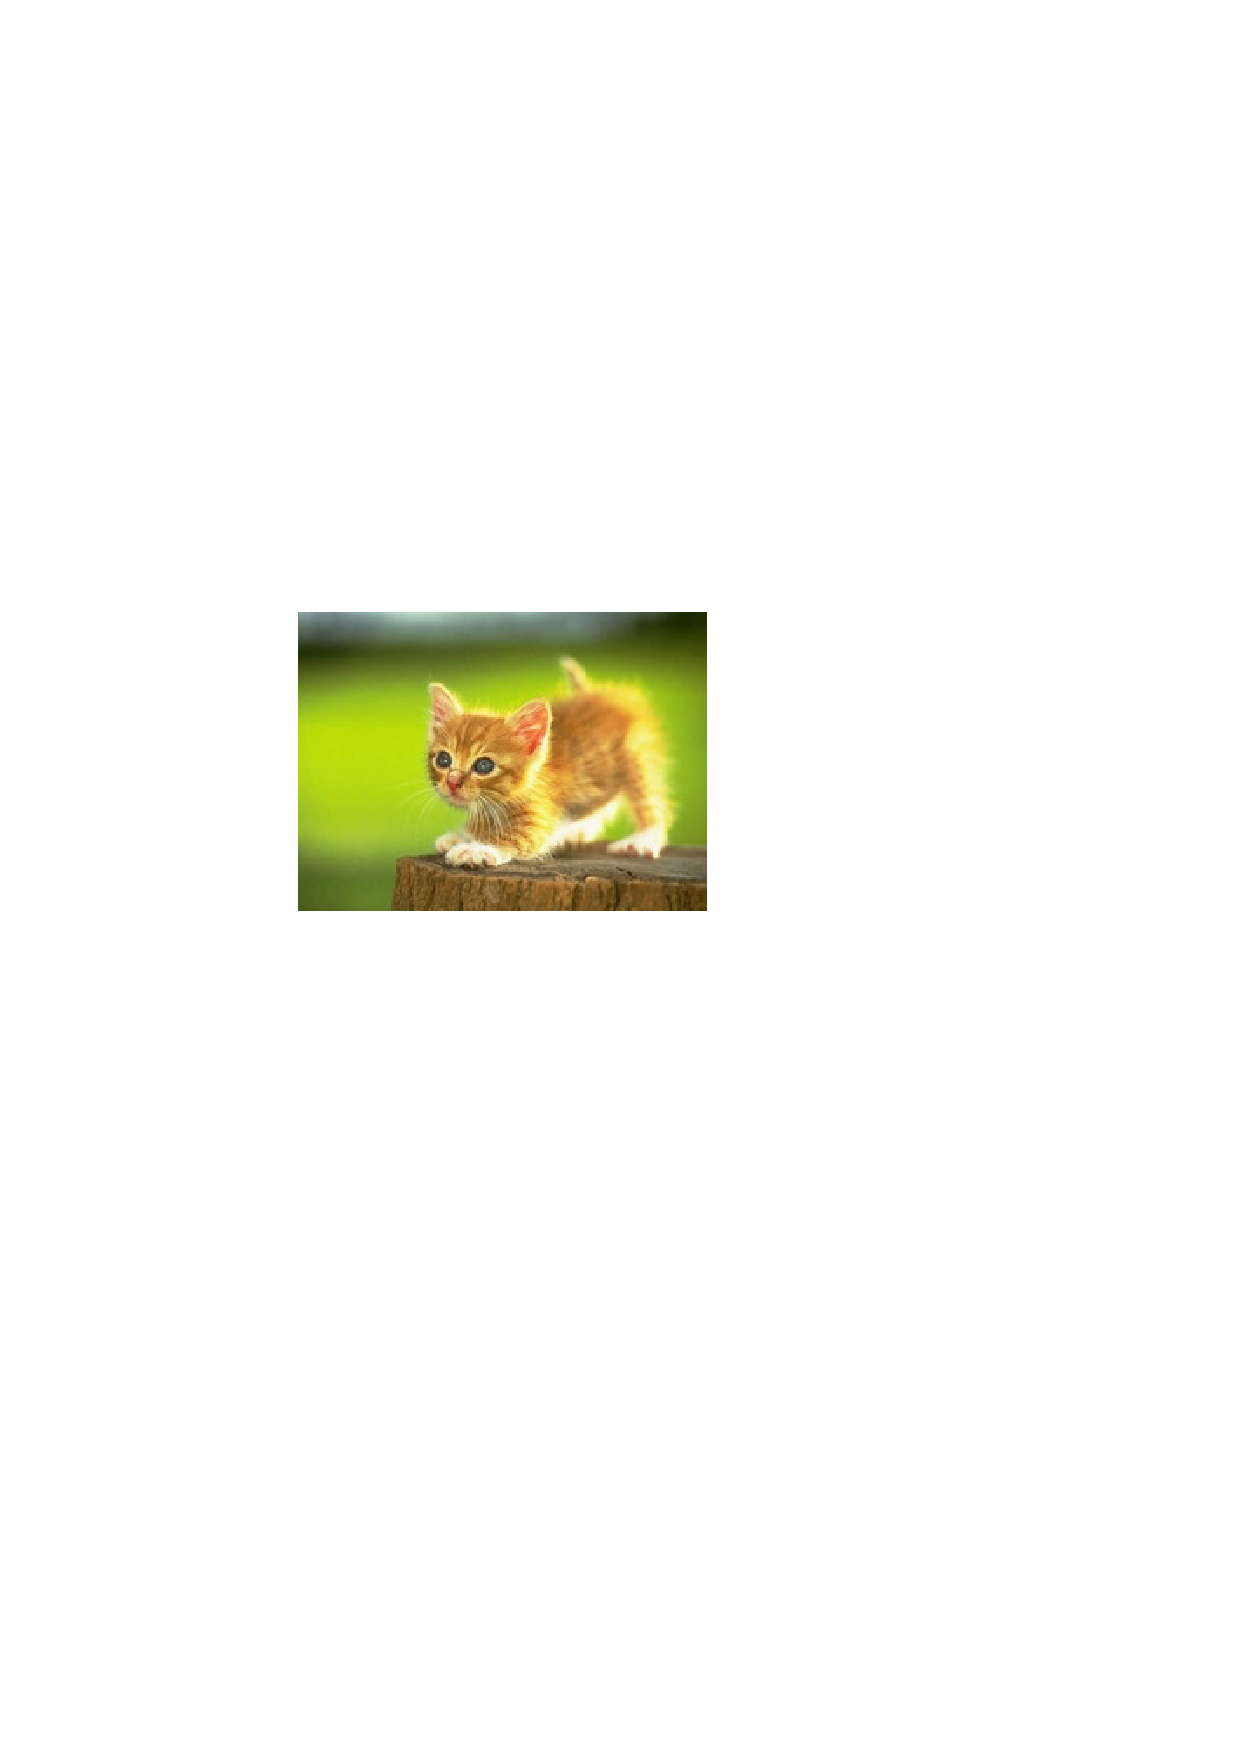
\includegraphics[width=\textwidth]{fig-example.pdf}
  \caption{Figure B}\label{fig:2-2}
  \end{subfigure}
\caption{Multi-figures}\label{fig:2}
\end{figure}

\section{Bibliography}
Cite one bib\cite{knuth}, cite two\cite{TEXGURU99,knuth}.

\section[\textbackslash{}autoref Test]{\texttt{\textbackslash{}autoref} Test}

\begin{description}
  \item[Equation] \autoref{eq:1}
  \item[Footnote] \autoref{footnote:1}
  \item[Item] \autoref{item:1},\autoref{item:2},\autoref{item:3}
  \item[Figure] \autoref{fig:1}
  \item[Table] \autoref{tab:1}
  \item[Appendix] \autoref{appendix:1}
  \item[Chapter] \autoref{chapter:1}
  \item[Section] \autoref{sec:1},\autoref{sec:2},\autoref{sec:3}
  \item[Algorithm] \autoref{alg:1},\autoref{alg_line:1}
  \item[Theorem] \autoref{def:1},\autoref{proposition:1},\autoref{axiom:1},\autoref{lemma:1},\autoref{theorem:1},\autoref{proof:1}
\end{description}

\backmatter

\begin{ack}
Acknowledge
\end{ack}

\bibliography{ref-example}

\appendix

\begin{publications}
    \item Thesis 1
    \item Thesis 2
\end{publications}

\chapter{This is an appendix}\label{appendix:1}
Content.


\end{document}
\endinput
%%
%% End of file `hustreport-en-example.tex'.
